\documentclass[conference]{IEEEtran}

% ------------------------------------------------------------------ paquetes
\usepackage[utf8]{inputenc}
\usepackage[T1]{fontenc}
\usepackage[spanish,es-noshorthands,es-tabla,es-nodecimaldot]{babel}
\usepackage{amsmath,amssymb}
\usepackage{icomma}
\usepackage{graphicx}
\usepackage{array}
\usepackage{cite}
\usepackage{xcolor}
\usepackage{listings}
\usepackage{tikz}
\usetikzlibrary{arrows.meta,positioning,calc}
\usepackage[european]{circuitikz}
\usepackage[hidelinks]{hyperref}

\addto\captionsspanish{\renewcommand{\figurename}{Fig.}}
\renewcommand{\arraystretch}{1.15}

\lstset{
  language=C++,
  basicstyle=\ttfamily\footnotesize,
  keywordstyle=\bfseries,
  commentstyle=\itshape\color{black!60},
  numbers=left, numberstyle=\tiny, numbersep=6pt,
  breaklines=true, frame=single, columns=fullflexible,
  tabsize=2, showstringspaces=false
}

\begin{document}

% ------------------------------------------------------------------ título
\title{Electroestimulador}

\author{
\IEEEauthorblockN{Javier Oliva, Matias Bustos, Barbara Pavez}
\IEEEauthorblockA{Escuela de Bioingeniería Médica, Facultad de Medicina, Universidad Católica del Maule\\
Talca, Chile\\
javier.oliva@alumnos.ucm.cl\\
matias.bustos@alumnos.ucm.cl\\
barbara.pavez@alumnos.ucm.cl}
}

\maketitle

% ------------------------------------------------------------------ resumen
\begin{abstract}
Se describe el diseño y montaje de un electroestimulador experimental de baja tensión, destinado únicamente a generar y estudiar las señales empleadas en electroestimulación, sin aplicarlas al cuerpo. Un temporizador NE555 en configuración astable genera una onda cuadrada cuya frecuencia y ciclo útil se ajustan con dos potenciómetros de 50~k$\Omega$ y un condensador de temporización de 2,2~$\mu$F. Un amplificador operacional LM324 convierte esa señal en una onda triangular mediante un seguidor de tensión y un integrador inversor con condensador de acople, resistencia de realimentación y voltaje de referencia ajustable. Un conmutador selecciona la forma de onda y un tercer potenciómetro, conectado como divisor de voltaje, fija su amplitud. El circuito se alimenta con los 5~V de un Arduino UNO y se aloja en una carcasa impresa en 3D con PLA, con forma de radio de los años 60. Las señales se midieron con un osciloscopio programado por el equipo sobre un Arduino UNO. Se obtuvo una frecuencia de 4,773 a 541,4~Hz, un ciclo útil de 49,6 a 99,3~\%, una onda cuadrada de hasta 4,1~Vpp y una onda triangular de 0,767~Vpp a 10,61~Hz, valores que concuerdan con los calculados con una diferencia de entre 0,4 y 9,4~\%. El error del instrumento de medición frente a un osciloscopio comercial no fue determinado.
\end{abstract}

\begin{IEEEkeywords}
Electroestimulación, NE555, multivibrador astable, LM324, integrador, onda triangular, Arduino.
\end{IEEEkeywords}

% ------------------------------------------------------------------ I
\section{Introducción}

\IEEEPARstart{L}{a} electroestimulación consiste en aplicar corrientes eléctricas de baja intensidad a los tejidos para provocar la respuesta de nervios o músculos. Se utiliza en rehabilitación, en el tratamiento del dolor y en el fortalecimiento muscular, y su efecto depende de tres parámetros de la señal: la frecuencia, la duración o ciclo útil de cada impulso y la amplitud \cite{low}.

El objetivo de este proyecto fue diseñar e implementar un generador de señales de bajo costo que permita controlar esos tres parámetros de forma independiente, entregar dos formas de onda, cuadrada y triangular, y observarlas en un osciloscopio. Para ello se emplearon un temporizador NE555, un amplificador operacional cuádruple LM324 y un Arduino UNO como fuente de alimentación e instrumento de medición. El dispositivo es didáctico: su salida no se conecta al cuerpo.

% ------------------------------------------------------------------ II
\section{Marco Teórico}

El NE555 es un temporizador integrado formado por dos comparadores, un biestable y un transistor de descarga \cite{ne555}. En configuración astable, una resistencia $R_A$ conecta la alimentación con el pin~7 (descarga), una resistencia $R_B$ une el pin~7 con los pines~6 y~2 (umbral y disparo), y un condensador $C_T$ conecta estos últimos con tierra. El condensador se carga a través de $R_A+R_B$ hasta $\tfrac{2}{3}V_{CC}$; en ese momento la salida (pin~3) pasa a nivel bajo y el condensador se descarga solo a través de $R_B$ hasta $\tfrac{1}{3}V_{CC}$, donde el ciclo se repite. Los tiempos en alto y en bajo son:
\begin{equation}
t_H = 0{,}693\,(R_A+R_B)\,C_T, \qquad t_L = 0{,}693\,R_B\,C_T
\end{equation}
por lo que la frecuencia y el ciclo útil resultan:
\begin{equation}
f = \frac{1}{t_H+t_L} = \frac{1{,}44}{(R_A+2R_B)\,C_T}
\label{eq:f}
\end{equation}
\begin{equation}
D = \frac{t_H}{t_H+t_L} = \frac{R_A+R_B}{R_A+2R_B}
\end{equation}
Como $t_H$ incluye a $R_A$, el ciclo útil es siempre mayor o igual que 50~\%. Además, $R_A$ y $R_B$ aparecen en ambas expresiones, de modo que el ajuste del ciclo útil también modifica la frecuencia.

La onda triangular se obtiene integrando la onda cuadrada. En un integrador inversor, la entrada inversora del amplificador se mantiene al voltaje $V_{ref}$ de la entrada no inversora; la corriente que entra por la resistencia $R$ carga el condensador de realimentación $C$, y la salida es \cite{sedra}:
\begin{equation}
v_o(t) = V_{ref} - \frac{1}{RC}\int \left(v_i(t)-V_{ref}\right)dt
\end{equation}
Si la entrada es una onda cuadrada sin componente continua, la salida cambia con pendiente constante en cada semiperíodo y forma una onda triangular. Para un ciclo útil de 50~\%, su amplitud pico a pico es:
\begin{equation}
V_{pp,tri} = \frac{V_{pp,cuad}\;T}{4RC}
\label{eq:tri}
\end{equation}
donde $T=1/f$ es el período. La amplitud de la triangular es, por lo tanto, inversamente proporcional a la frecuencia.

Un integrador ideal tiene ganancia infinita en continua, por lo que cualquier desbalance lo lleva a saturación. Para evitarlo se coloca una resistencia $R_f$ en paralelo con $C$, que limita la ganancia en continua a $R_f/R$ y solo afecta a la integración por debajo de:
\begin{equation}
f_{R_f} = \frac{1}{2\pi R_f C}
\end{equation}
Asimismo, un condensador de acople $C_a$ en serie con $R$ elimina la componente continua de la onda cuadrada. Como la entrada inversora es una tierra virtual, $C_a$ y $R$ forman un filtro pasa altos con frecuencia de corte:
\begin{equation}
f_c = \frac{1}{2\pi R\,C_a}
\end{equation}

Antes del integrador se ubica un seguidor de tensión, de ganancia unitaria, alta impedancia de entrada y baja impedancia de salida, que entrega la corriente que exige el integrador sin cargar al 555.

La amplitud se controla con un potenciómetro $R_P$ conectado como divisor de voltaje. Si $\alpha$ es la fracción del recorrido entre el cursor y tierra:
\begin{equation}
v_{out} = \alpha\,v_{in}, \qquad R_{th} = \alpha\,(1-\alpha)\,R_P
\end{equation}
donde $R_{th}$ es la resistencia de salida del divisor, cuyo valor máximo es $R_P/4$ en la mitad del recorrido.

Las señales se miden con el conversor analógico-digital de 10 bits del Arduino UNO, cuyo voltaje se obtiene como $V = 5\,c/1023$, donde $c$ es la cuenta entregada por el conversor, lo que equivale a unos 4,9~mV por cuenta \cite{atmega}. Para que el conversor lea correctamente, la fuente conectada a la entrada debe tener una impedancia de 10~k$\Omega$ o menos, y la frecuencia de muestreo debe ser mayor que el doble de la frecuencia de la señal.

% ------------------------------------------------------------------ III
\section{Descripción de producto}

El electroestimulador es un generador de señales de baja tensión con dos formas de onda. Un oscilador NE555 produce una onda cuadrada que se divide en dos ramas: una la lleva directamente a la salida y la otra la transforma en una onda triangular mediante un LM324. Un conmutador interior selecciona la rama y un potenciómetro final fija la amplitud de la señal, que se observa en un osciloscopio.

El circuito se encuentra en una carcasa de PLA impresa en 3D, de $180 \times 72 \times 105$~mm, con forma de radio de los años 60: asa, dial y rejilla en el frente. Los tres mandos se ubican en columna a la derecha: amplitud (P3) arriba, ciclo útil (P2) al centro y frecuencia (P1) abajo. Para funcionar requiere los 5~V de un Arduino UNO conectado por USB a un computador. Tres cables salen por la tapa trasera: alimentación (+5~V), tierra y señal, cada uno por una ranura con su símbolo grabado.

\begin{figure}[!t]
\centering
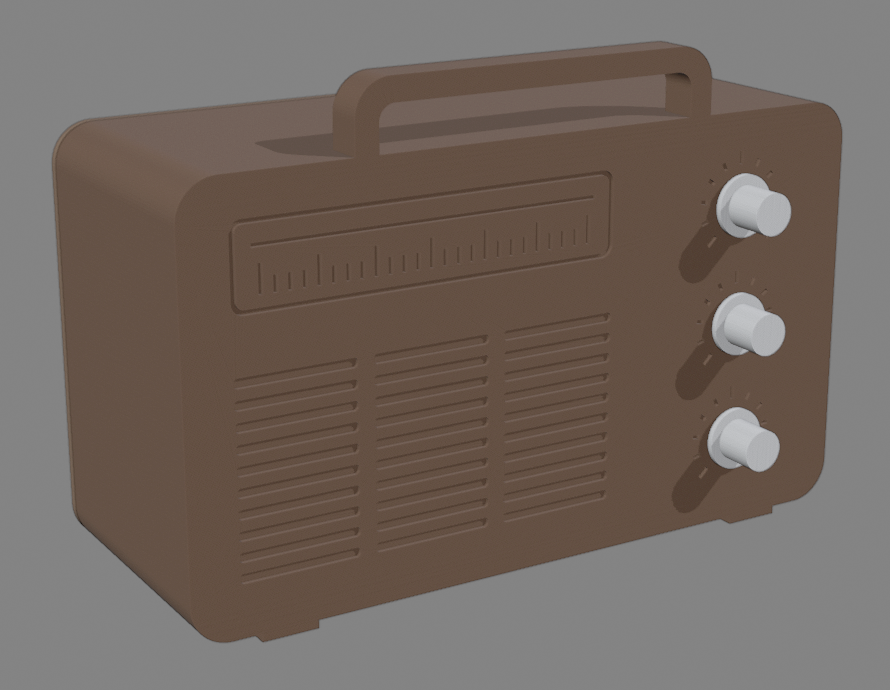
\includegraphics[width=0.92\columnwidth]{figuras/producto.png}
\caption{Electroestimulador desarrollado: carcasa con forma de radio impresa en 3D, con el dial, la rejilla y los mandos de amplitud, ciclo útil y frecuencia.}
\label{fig:producto}
\end{figure}

% ------------------------------------------------------------------ IV
\section{Diseño}

\subsection{Componentes}

El electroestimulador se diseñó a partir de una etapa de oscilación, una etapa de integración, una etapa de selección y control de amplitud y un sistema de medición. La Fig.~\ref{fig:bloques} presenta su diagrama de bloques.

\begin{figure}[!t]
\centering
\resizebox{\columnwidth}{!}{%
\begin{tikzpicture}[
  font=\footnotesize,
  blk/.style={draw, thick, rounded corners=2pt, align=center, minimum height=8mm, minimum width=19mm, fill=black!4},
  >={Stealth[length=2mm]}, node distance=4mm and 6mm]
\node[blk] (osc) {Oscilador\\NE555 astable};
\node[blk, above right=1mm and 7mm of osc] (seg) {Seguidor\\LM324 A};
\node[blk, right=of seg] (int) {Integrador\\LM324 C};
\node[blk, below right=1mm and 7mm of osc, minimum width=44mm] (cua) {Rama cuadrada (directa)};
\coordinate (mid) at ($(int.east)!0.5!(cua.east)$);
\node[blk, right=8mm of mid, minimum width=12mm] (sw) {SW1};
\node[blk, below=6mm of sw, minimum width=12mm] (amp) {P3\\amplitud};
\node[left=8mm of amp, align=center] (sal) {Salida\\(A0)};
\draw[->] (osc.east) -- ++(3mm,0) |- (seg.west);
\draw[->] (osc.east) -- ++(3mm,0) |- (cua.west);
\draw[->] (seg) -- (int);
\draw[->] (int.east) -- ++(2mm,0) |- ([yshift=1.5mm]sw.west);
\draw[->] (cua.east) -- ++(2mm,0) |- ([yshift=-1.5mm]sw.west);
\draw[->] (sw) -- (amp);
\draw[->] (amp) -- (sal);
\node[above=0mm of osc, font=\scriptsize] {P1, P2, $C_T$};
\node[above=0mm of int, font=\scriptsize] {VR4 (centrado)};
\end{tikzpicture}}
\caption{Diagrama de bloques del electroestimulador: la onda cuadrada del oscilador se divide en dos ramas, el conmutador elige una y el mando de amplitud fija su altura antes de la salida.}
\label{fig:bloques}
\end{figure}

La Tabla~\ref{tab:componentes} presenta los componentes utilizados. Los potenciómetros, resistencias y condensadores son genéricos, por lo que sus valores corresponden a los nominales y tienen la tolerancia propia de cada tipo.

\begin{table}[!t]
\caption{Componentes del proyecto}
\label{tab:componentes}
\centering
\begin{tabular}{>{\raggedright\arraybackslash}p{0.30\columnwidth} >{\raggedright\arraybackslash}p{0.60\columnwidth}}
\hline
\textbf{Componente} & \textbf{Característica} \\
\hline
NE555 & Temporizador en configuración astable, alimentado a 5~V \\
LM324 & Cuatro amplificadores operacionales: A como seguidor, C como integrador; B y D como seguidores con la entrada no inversora a GND \\
P1 ($R_A$) & Potenciómetro de 50~k$\Omega$ lineal, entre +5~V y el pin~7: frecuencia \\
P2 ($R_B$) & Potenciómetro de 50~k$\Omega$ lineal, entre el pin~7 y los pines~6 y~2: ciclo útil \\
P3 & Potenciómetro de 10~k$\Omega$ lineal, como divisor de voltaje: amplitud \\
$C_T$ & 2,2~$\mu$F, entre los pines~6 y~2 y GND \\
Condensador del pin~5 & 10~nF a GND, estabiliza los umbrales del 555 \\
Integrador & $C_a = 10~\mu$F (acople), $R = 10$~k$\Omega$, $C = 10~\mu$F, $R_f = 220$~k$\Omega$; condensadores cerámicos «106» \\
Referencia & VR4 de 10~k$\Omega$ entre +5~V y GND; cursor a la entrada no inversora por 100~k$\Omega$ \\
SW1 & Conmutador de tres terminales: selección de onda \\
Mandos & Potenciómetros WH148 de 16~mm con perillas \\
Carcasa & Impresión 3D con PLA, $180 \times 72 \times 105$~mm, sin tornillos \\
Alimentación & 5~V del Arduino UNO vía USB, con tierra común \\
Instrumento & Osciloscopio programado sobre un Arduino UNO \\
\hline
\end{tabular}
\end{table}

\subsection{Etapa de oscilación}

El NE555 se conectó en configuración astable. El potenciómetro P1, conectado como resistencia variable, cumple la función de $R_A$ entre +5~V y el pin~7, y el potenciómetro P2 cumple la de $R_B$ entre el pin~7 y los pines~6 y~2, unidos entre sí. El condensador $C_T$ de 2,2~$\mu$F une los pines~6 y~2 con tierra. Los pines~4 (reinicio) y~8 (alimentación) se conectan a +5~V, el pin~1 a tierra y el pin~5 a un condensador de 10~nF hacia tierra, que estabiliza los umbrales internos.

Con $R_A$ y $R_B$ de 50~k$\Omega$ como máximo, la ecuación~\eqref{eq:f} entrega una frecuencia mínima de 4,36~Hz con ambos potenciómetros al máximo. El ciclo útil va desde 50~\% con $R_A \approx 0$ hasta casi 100~\% con $R_B \approx 0$. La salida del 555, el pin~3, alimenta a las dos ramas al mismo tiempo.

\subsection{Etapa de integración}

La rama triangular comienza en un seguidor de tensión, formado por el amplificador A del LM324: la señal entra por el pin~3 (no inversor) y la salida, el pin~1, se une al pin~2 (inversor).

La salida del seguidor pasa por el condensador de acople $C_a$ de 10~$\mu$F y la resistencia $R$ de 10~k$\Omega$ antes de llegar al pin~9, la entrada inversora del amplificador C. Entre el pin~9 y la salida, el pin~8, se conectan en paralelo el condensador $C$ de 10~$\mu$F y la resistencia $R_f$ de 220~k$\Omega$. Con estos valores, $RC = 0{,}1$~s; $R_fC = 2{,}2$~s, la ganancia en continua queda limitada a 22 y $f_{R_f} = 0{,}072$~Hz. El acople tiene una frecuencia de corte de 1,6~Hz.

El LM324 funciona con una sola fuente de 5~V, por lo que su salida solo puede variar entre 0 y unos 3,5~V \cite{lm324}. Por esta razón, la entrada no inversora, el pin~10, recibe un voltaje de referencia desde el cursor del potenciómetro VR4, conectado entre +5~V y tierra, a través de una resistencia de 100~k$\Omega$. La onda triangular queda centrada en ese voltaje.

Durante el montaje se encontraron y corrigieron cuatro problemas: un primer integrador armado con el condensador en el camino de la señal, que se comportaba como derivador; una salida recortada en 0~V por tener la entrada no inversora a tierra; la saturación del integrador por la componente continua de la onda cuadrada, que se resolvió con el condensador de acople; y una segunda etapa de integración que entregaba curvas casi senoidales, por lo que se eliminó. Los amplificadores B y D, que no se usan, se conectaron como seguidores con su entrada no inversora a tierra para evitar que oscilen y agreguen ruido a la alimentación común. El LM324 se alimenta por el pin~4 (+5~V) y el pin~11 (tierra).

\subsection{Selección de onda y control de amplitud}

Las dos ramas llegan al conmutador SW1, ubicado en el interior de la carcasa: su terminal izquierdo recibe la onda triangular desde el pin~8 del LM324, el derecho recibe la onda cuadrada desde el pin~3 del 555, y el central entrega la onda seleccionada.

El terminal central se conecta a un extremo del potenciómetro P3, cuyo otro extremo va a tierra; su cursor es la salida del dispositivo. Al ubicarse al final, P3 regula por igual ambas formas de onda y no interviene en la red de tiempo del 555, por lo que no modifica la frecuencia. Con 10~k$\Omega$, la resistencia de salida no supera los 2,5~k$\Omega$, valor adecuado para la entrada del Arduino.

Los mandos P1, P2 y P3 se montaron en el frente de la carcasa. El conmutador SW1 y el potenciómetro de centrado VR4 quedan en la miniplaca interior, accesibles al retirar la tapa trasera.

\subsection{Sistema de medición}

Las señales se midieron con un osciloscopio desarrollado por el equipo, compuesto por un programa para Arduino UNO y una interfaz web que se abre en Chrome o Edge. El programa, cuyo código se incluye al final del informe, utiliza el Timer1 para marcar el instante de cada muestra y el conversor de 10 bits para digitalizar las entradas A0 a A5. Dispone de un modo ráfaga, que almacena hasta 1800 bytes en memoria con disparo y pre-disparo a una frecuencia de hasta 100~000 muestras por segundo, y de un modo continuo, que envía las muestras a medida que se toman. La comunicación con el computador se realiza a 500~000 baudios.

La interfaz calcula el voltaje pico a pico, máximo, mínimo, medio y eficaz, la frecuencia, el período y el ciclo útil. También ofrece vistas de espectro (FFT) y X-Y, cursores, exportación de los datos en CSV o PNG, y un modo de demostración sin placa.

% ------------------------------------------------------------------ V
\section{Manual de usuario}

\subsection{Descripción general}

El electroestimulador es un dispositivo de uso académico diseñado para generar ondas cuadradas y triangulares de baja tensión y estudiar los parámetros que se utilizan en electroestimulación. Dispone de tres mandos frontales para la frecuencia (P1), el ciclo útil (P2) y la amplitud (P3), un conmutador interior de forma de onda y un ajuste interior de centrado de la onda triangular.

Para su funcionamiento, el dispositivo requiere los 5~V de un Arduino UNO conectado por USB a un computador. La señal se observa con el osciloscopio Arduino o con cualquier osciloscopio que admita señales de 0 a 5~V.

\subsection{Procedimiento de operación}

Antes de comenzar, se debe comprobar que el equipo se encuentre sobre una superficie estable, limpia y seca, y que el Arduino esté desconectado del computador.

\textit{Conexión de los cables.} Conectar el cable marcado con «+» al pin de 5~V del Arduino, el marcado con «$-$» a GND y el cable de señal a la entrada A0.

\textit{Encendido.} Conectar el Arduino al computador mediante USB. Abrir la interfaz del osciloscopio en Chrome o Edge y presionar «Conectar Arduino». Si se necesita verificar la interfaz sin el circuito, el botón «Demo sin placa» genera una señal de prueba.

\textit{Selección de la forma de onda.} Con el Arduino desconectado, retirar la tapa trasera y colocar el conmutador interior en la posición de onda cuadrada o triangular. Volver a colocar la tapa a presión antes de reconectar.

\textit{Ajuste de la frecuencia.} Girar el mando inferior (P1) hasta obtener la frecuencia deseada, que la interfaz muestra en la barra de mediciones.

\textit{Ajuste del ciclo útil.} Girar el mando central (P2). Como este mando también modifica la frecuencia, se recomienda ajustar primero el ciclo útil y luego corregir la frecuencia con P1.

\textit{Ajuste de la amplitud.} Girar el mando superior (P3) hasta obtener la amplitud deseada. Este mando no modifica la frecuencia ni el ciclo útil.

\textit{Centrado de la onda triangular.} Si la onda triangular aparece recortada, desconectar el Arduino, retirar la tapa y girar lentamente el potenciómetro de centrado VR4 de la miniplaca. Repetir hasta que la onda quede completa en la pantalla.

\textit{Lectura.} Para señales lentas, usar el modo continuo; para señales rápidas, el modo ráfaga, que muestrea a mayor velocidad. El botón «Autoajuste» selecciona una escala adecuada. Los valores de voltaje, frecuencia, período y ciclo útil aparecen bajo la pantalla del osciloscopio.

\subsection{Interpretación de resultados}

La interfaz del osciloscopio presenta, entre otras, las siguientes magnitudes:

\textit{Frecuencia ($f$) y período ($T$):} número de ciclos por segundo y duración de cada ciclo, relacionados por $T = 1/f$.

\textit{Ciclo útil ($D$):} porcentaje del período en que la onda cuadrada permanece en nivel alto. En este circuito es siempre mayor o igual que 50~\%.

\textit{Voltaje pico a pico ($V_{pp}$):} diferencia entre el valor máximo y el mínimo de la señal; es la magnitud que regula P3.

En la onda triangular, la amplitud disminuye al aumentar la frecuencia, según la ecuación~\eqref{eq:tri}. Por ello, para comparar amplitudes de la triangular se debe indicar siempre a qué frecuencia se midieron.

\subsection{Comportamiento de la señal y solución de problemas}

Durante la operación pueden observarse los siguientes comportamientos:

\textit{Onda triangular recortada por abajo o por arriba.} La señal alcanza el límite de 0~V o de unos 3,5~V del LM324. Ajustar el centrado con VR4.

\textit{Onda triangular muy pequeña.} La frecuencia es alta. Disminuir la frecuencia con P1 o reducir la escala de voltios por división.

\textit{Onda triangular deformada o trapezoidal.} Por debajo de unos 3~Hz, la amplitud calculada supera el rango de salida del LM324 y la onda se recorta. Aumentar la frecuencia.

\textit{El ciclo útil no baja del 50~\%.} Es una limitación propia de la configuración astable, no una falla.

\textit{La frecuencia cambia al mover P2.} Es el comportamiento esperado, porque $R_B$ interviene en la frecuencia. Corregirla con P1.

\textit{No aparece señal.} Verificar la conexión de los tres cables y la alimentación de 5~V, y que P3 no esté al mínimo, donde solo queda un residuo de unos 15~mVpp.

\textit{Onda rápida con forma irregular.} En el modo continuo, la frecuencia de muestreo puede ser insuficiente para la señal. Cambiar al modo ráfaga.

\subsection{Precauciones de uso}

\textit{Uso exclusivamente didáctico.} El dispositivo no tiene aislamiento galvánico, limitación de corriente ni salida bifásica sin componente continua. Su salida no debe conectarse al cuerpo ni a electrodos.

\textit{Alimentación eléctrica.} Utilizar únicamente los 5~V del Arduino o una fuente de 5~V regulada, comprobando la polaridad antes de conectar. No aplicar voltajes mayores, ya que la señal se conecta directamente a la entrada A0, que no admite más de 5~V ni voltajes negativos.

\textit{Intervenciones.} Desconectar el Arduino del computador antes de retirar la tapa, mover el conmutador interior o ajustar VR4. No modificar componentes ni conexiones con el circuito alimentado.

\textit{Conservación de la carcasa.} Debido a que la estructura está fabricada con PLA, se recomienda evitar temperaturas elevadas, la exposición prolongada al sol, golpes y esfuerzos que puedan deformarla o soltar los potenciómetros de sus patillas de sujeción.

\subsection{Apagado y almacenamiento}

Una vez finalizadas las mediciones, presionar el botón de detención de la interfaz, desconectar el Arduino del computador y luego los tres cables del dispositivo.

Se recomienda almacenar el equipo en un lugar protegido de la humedad, el polvo y las fuentes de calor, sin peso sobre los mandos.

% ------------------------------------------------------------------ VI
\section{Datasheet}

\subsection{Descripción}

El dispositivo desarrollado corresponde a un electroestimulador didáctico de bajo costo, diseñado para generar ondas cuadradas y triangulares con frecuencia, ciclo útil y amplitud ajustables. Utiliza un temporizador NE555 como oscilador y un amplificador LM324 como seguidor e integrador, y se alimenta con los 5~V de un Arduino UNO, que también puede adquirir su señal.

\subsection{Especificaciones}

\begin{table}[!t]
\caption{Especificaciones del electroestimulador}
\label{tab:especificaciones}
\centering
\begin{tabular}{>{\raggedright\arraybackslash}p{0.33\columnwidth} >{\raggedright\arraybackslash}p{0.57\columnwidth}}
\hline
\textbf{Parámetro} & \textbf{Especificación} \\
\hline
Alimentación & 5~V c.c. desde el Arduino UNO (USB), tierra común \\
Consumo de corriente & No medido \\
Oscilador & NE555 en configuración astable \\
Formas de onda & Cuadrada o triangular, según SW1 \\
Frecuencia & 4,773 a 541,4~Hz (medida) \\
Ciclo útil & 49,6 a 99,3~\% (medido) \\
Amplitud de la cuadrada & 0 a 4,1~Vpp aprox., ajustable con P3 \\
Residuo con P3 al mínimo & 14,6~mVpp \\
Onda triangular & 0,767~Vpp a 10,61~Hz, centrada en 1,3~V (ajustable con VR4) \\
Integrador & $RC = 0{,}1$~s; $R_fC = 2{,}2$~s; ganancia en continua 22 \\
Corte del acople & 1,6~Hz \\
Amplificador & LM324, dos de sus cuatro amplificadores en uso \\
Resistencia de salida & 2,5~k$\Omega$ como máximo (P3 de 10~k$\Omega$) \\
Mandos & P1 frecuencia, P2 ciclo útil, P3 amplitud \\
Ajustes interiores & Conmutador de onda (SW1) y centrado (VR4) \\
Conexiones & Tres cables por la tapa trasera: +5~V, GND y señal \\
Material de carcasa & PLA impreso en 3D, ensamble a presión \\
Dimensiones & $180 \times 72 \times 105$~mm, sin asa ni patas \\
\hline
\end{tabular}
\end{table}

La Tabla~\ref{tab:especificaciones} resume las especificaciones del dispositivo. Los valores de frecuencia, ciclo útil y amplitud corresponden a los medidos con el osciloscopio Arduino.

\subsection{Circuito interno}

El funcionamiento del dispositivo comienza en el NE555, que genera la onda cuadrada con la frecuencia y el ciclo útil fijados por P1, P2 y $C_T$. Su salida alimenta la rama cuadrada, que llega directamente al conmutador, y la rama triangular, que pasa por el seguidor y el integrador del LM324.

La Fig.~\ref{fig:esquema} muestra el esquemático del circuito. P1 conecta +5~V con el pin~7 del 555, P2 une el pin~7 con los pines~6 y~2, y $C_T$ une estos últimos con tierra. El pin~3 se conecta al terminal derecho de SW1 y a la entrada no inversora del seguidor, el pin~3 del LM324. La salida del seguidor llega al integrador a través de $C_a$ y $R$, y la salida del integrador, el pin~8, al terminal izquierdo de SW1. El terminal central de SW1 va a P3, cuyo cursor es la salida. Todo el circuito se alimenta con los 5~V del Arduino y comparte su tierra.

\begin{figure*}[!t]
\centering
\begin{circuitikz}[scale=0.82, transform shape, font=\footnotesize]
  % ---------------- NE555
  \draw[thick] (3,0) rectangle (5.4,4);
  \node at (4.2,2.9) {\textbf{NE555}};
  \node[right, font=\scriptsize] at (3,3.2) {7};
  \node[right, font=\scriptsize] at (3,2.0) {6};
  \node[right, font=\scriptsize] at (3,1.2) {2};
  \node[below, font=\scriptsize] at (3.6,4) {8};
  \node[below, font=\scriptsize] at (4.8,4) {4};
  \node[above, font=\scriptsize] at (3.6,0) {1};
  \node[above, font=\scriptsize] at (4.8,0) {5};
  \node[left,  font=\scriptsize] at (5.4,2.4) {3};
  % pines 8 y 4 a +5 V
  \draw (3.6,4) -- (3.6,4.6) -- (4.8,4.6) -- (4.8,4);
  \draw (4.2,4.6) node[vcc]{+5\,V};
  % pin 1 a GND, pin 5 con 10 nF
  \draw (3.6,0) -- (3.6,-0.4) node[ground]{};
  \draw (4.8,0) to[C, l=10\,nF] (4.8,-1.6) node[ground]{};
  % red de tiempo
  \draw (1.2,5.4) node[vcc]{+5\,V} to[vR, l_={$P_1$ 50\,k$\Omega$}] (1.2,3.2);
  \draw (1.2,3.2) to[short, *-] (3,3.2);
  \draw (1.2,3.2) to[vR, l_={$P_2$ 50\,k$\Omega$}] (1.2,1.2);
  \draw (1.2,1.2) to[short, *-] (3,1.2);
  \draw (3,2.0) -- (2.5,2.0) to[short, -*] (2.5,1.2);
  \draw (1.2,1.2) to[C, l_={$C_T$ 2,2\,$\mu$F}] (1.2,-0.6) node[ground]{};
  % salida del 555
  \draw (5.4,2.4) to[short, -*] (6.4,2.4) coordinate (n3);
  % ---------------- seguidor (LM324 A)
  \node[op amp, noinv input up, anchor=+] (OA1) at (7.4,2.4) {};
  \node[font=\scriptsize] at ($(OA1)+(0.1,0.75)$) {U2A};
  \draw (n3) -- (OA1.+);
  \node[above left, font=\scriptsize] at (OA1.+) {3};
  \node[below left, font=\scriptsize] at (OA1.-) {2};
  \node[above right, font=\scriptsize] at (OA1.out) {1};
  \draw (OA1.-) -- ++(-0.3,0) |- ($(OA1.out)+(0.25,-1.0)$) -- ($(OA1.out)+(0.25,0)$);
  \draw (OA1.out) to[short, -*] ($(OA1.out)+(0.25,0)$) coordinate (aout);
  % acople y resistencia de entrada
  \draw (aout) to[C, l={$C_a$ 10\,$\mu$F}] ++(1.8,0) to[R, l={$R$ 10\,k$\Omega$}] ++(1.8,0) coordinate (rin);
  % ---------------- integrador (LM324 C)
  \node[op amp, anchor=-] (OA3) at ($(rin)+(0.9,0)$) {};
  \node[font=\scriptsize] at ($(OA3)+(0.1,0.75)$) {U2C};
  \draw (rin) to[short, -*] ($(rin)+(0.45,0)$) coordinate (fb) -- (OA3.-);
  \node[above right, font=\scriptsize] at ($(OA3.-)+(-0.1,0)$) {9};
  \node[below right, font=\scriptsize] at ($(OA3.+)+(-0.1,0)$) {10};
  \node[below right, font=\scriptsize] at (OA3.out) {8};
  \draw (OA3.out) to[short, -*] ($(OA3.out)+(0.4,0)$) coordinate (cout);
  \draw (fb) -- ++(0,1.3) coordinate (f1) to[C, l={$C$ 10\,$\mu$F}] (f1 -| cout) -- (cout);
  \draw (f1) -- ++(0,1.2) coordinate (f2) to[R, l={$R_f$ 220\,k$\Omega$}] (f2 -| cout) -- (f1 -| cout);
  % referencia (VR4)
  \draw (OA3.+) -- ++(-0.6,0) coordinate (pp) to[R, l_={100\,k$\Omega$}] ++(0,-1.8) coordinate (wp);
  \draw ($(wp)+(-1.4,1.0)$) node[vcc]{+5\,V} to[pR, n=vr4, l_={VR4 10\,k$\Omega$}] ($(wp)+(-1.4,-1.0)$) node[ground]{};
  \draw (vr4.wiper) -- (wp);
  % ---------------- SW1 y P3
  \coordinate (swc) at ($(cout)+(2.0,1.2)$);
  \coordinate (tt) at ($(swc)+(-1.0,-0.45)$);
  \draw (cout) -| (tt);
  \draw (n3) |- ($(swc)+(-1.0,3.2)$) |- ($(swc)+(-1.0,0.45)$) coordinate (tc);
  \fill (tt) circle (1.6pt) (tc) circle (1.6pt);
  \draw (swc) circle (1.6pt);
  \draw (swc) -- ($(tt)+(0.05,0.08)$);
  \node[font=\scriptsize] at ($(swc)+(0.5,-0.35)$) {SW1};
  \node[font=\scriptsize, right] at ($(tc)+(0,0.3)$) {cuadrada};
  \node[font=\scriptsize, right] at ($(tt)+(0,-0.35)$) {triangular};
  \draw (swc) -- ++(1.0,0) coordinate (p3t) to[pR, n=p3, l_={$P_3$ 10\,k$\Omega$}] ++(0,-2.4) node[ground]{};
  \draw (p3.wiper) -- ++(0.9,0) node[ocirc]{} node[right, align=left]{Salida\\(A0)};
\end{circuitikz}
\caption{Esquemático del circuito interno del electroestimulador. No se dibujan los amplificadores B y D del LM324, conectados como seguidores con la entrada no inversora a GND, ni la alimentación del LM324 (pin~4 a +5~V y pin~11 a GND).}
\label{fig:esquema}
\end{figure*}

\subsection{Rango de señal}

El instrumento entrega una onda cuadrada de 4,773 a 541,4~Hz con un ciclo útil de 49,6 a 99,3~\%, y una onda triangular obtenida de ella. La selección se realiza con el conmutador interior, y la amplitud de cualquiera de las dos ondas se regula con P3 desde unos 15~mVpp hasta su valor máximo.

A diferencia de un electroestimulador comercial, el prototipo no entrega impulsos bifásicos ni controla la corriente aplicada; sus señales son unipolares y de 0 a 5~V como máximo. La onda triangular conserva su forma desde unos 3~Hz, por debajo de los cuales se recorta, y su amplitud disminuye al subir la frecuencia, por lo que a las frecuencias más altas resulta muy pequeña.

\subsection{Consideraciones de uso}

El equipo debe operarse con los 5~V del Arduino, desconectándolo antes de abrir la tapa trasera. Su salida es solo para observación con un osciloscopio y nunca debe conectarse al cuerpo. Las precauciones eléctricas y de conservación de la carcasa se detallan en la sección V-E del manual de usuario.

% ------------------------------------------------------------------ VII
\section{Resultados}

\subsection{Procedimiento experimental}

Se conectó la salida del dispositivo a la entrada A0 del osciloscopio Arduino. Con la onda cuadrada seleccionada, se llevaron P1 y P2 a sus extremos para registrar la frecuencia y el ciclo útil mínimos y máximos, y se midió la amplitud de la cuadrada con P3 al máximo y al mínimo. Luego se seleccionó la onda triangular, se centró con VR4 y se midió su amplitud a 10,61~Hz en modo continuo, a 2000 muestras por segundo (Fig.~\ref{fig:triangular}). La Tabla~\ref{tab:resultados} resume los valores medidos y los compara con los calculados con las ecuaciones de la sección~II.

\begin{table}[!t]
\caption{Valores medidos y calculados}
\label{tab:resultados}
\centering
\begin{tabular}{>{\raggedright\arraybackslash}p{0.30\columnwidth} c c c}
\hline
\textbf{Parámetro} & \textbf{Medido} & \textbf{Calculado} & \textbf{Dif.} \\
\hline
Frecuencia mínima & 4,773~Hz & 4,36~Hz & +9,4~\% \\
Frecuencia máxima & 541,4~Hz & --- & --- \\
Ciclo útil mínimo & 49,6~\% & 50~\% & $-0{,}4$~pt \\
Ciclo útil máximo & 99,3~\% & $\to 100$~\% & --- \\
Cuadrada máxima & 4,1~Vpp & --- & --- \\
Residuo con P3 al mín. & 14,6~mVpp & 0 & --- \\
Triangular (10,61~Hz) & 0,767~Vpp & 0,825~Vpp & $-7{,}0$~\% \\
\hline
\end{tabular}
\end{table}

\begin{figure}[!t]
\centering
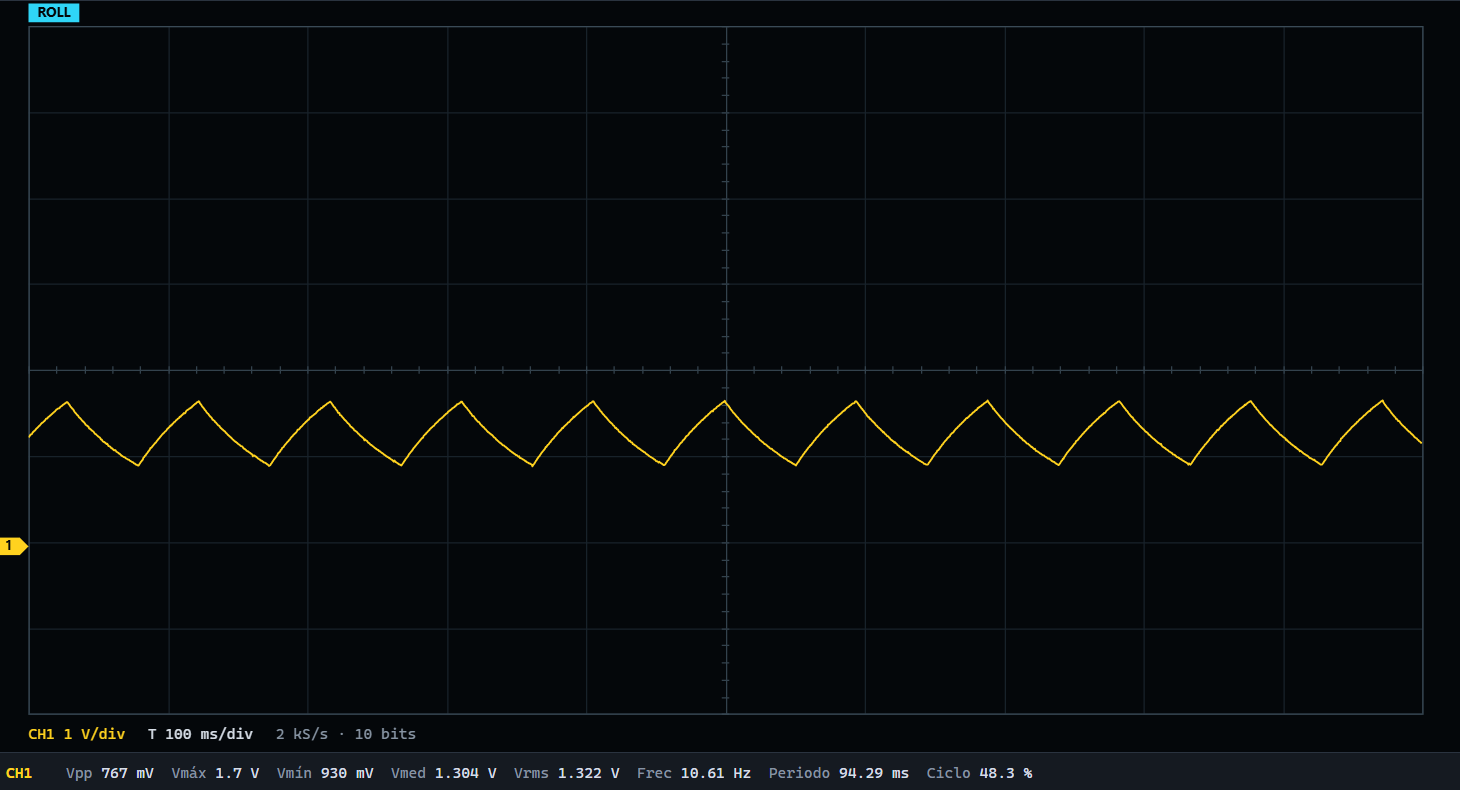
\includegraphics[width=\columnwidth]{figuras/triangular.png}
\caption{Onda triangular a la salida del integrador, medida con el osciloscopio Arduino en modo continuo: 0,767~Vpp, 10,61~Hz y valor medio de 1,304~V.}
\label{fig:triangular}
\end{figure}

\subsection{Análisis}

La frecuencia mínima medida, 4,773~Hz, supera en 9,4~\% a la calculada con potenciómetros de 50~k$\Omega$ y $C_T = 2{,}2~\mu$F. La diferencia es compatible con la tolerancia de los potenciómetros genéricos, habitualmente de $\pm 20$~\%, y de los condensadores cerámicos: el valor medido equivale a unos 46~k$\Omega$ por potenciómetro.

La frecuencia máxima, 541,4~Hz, no depende de los valores nominales sino de la resistencia que queda en los potenciómetros al llegar a su extremo. Según la ecuación~\eqref{eq:f}, corresponde a $R_A + 2R_B \approx 1{,}2$~k$\Omega$. Del mismo modo, el ciclo útil mínimo de 49,6~\% confirma que $R_A$ llega casi a cero, y el máximo de 99,3~\% indica que $R_B$ conserva unos cientos de ohmios en su extremo.

Para la onda triangular, la cuadrada que entrega el seguidor alcanza unos 3,5~Vpp, limitada por la salida del LM324. Con $T = 94{,}29$~ms y $RC = 0{,}1$~s, la ecuación~\eqref{eq:tri} da 0,825~Vpp, un 7~\% más que lo medido. La diferencia se explica porque el condensador de acople y $R_f$ restan una pequeña parte de cada rampa, y porque el ciclo útil de la señal no era exactamente 50~\%. La onda quedó centrada en 1,304~V, dentro del rango de salida del amplificador.

El residuo de 14,6~mVpp con P3 al mínimo equivale a unas 3 cuentas del conversor, por lo que se encuentra en el límite de resolución del instrumento.

Como no se contó con un osciloscopio comercial de referencia, estos resultados confirman el funcionamiento del circuito y su concordancia con la teoría, pero no permiten establecer la exactitud del instrumento de medición.

% ------------------------------------------------------------------ VIII
\section{Conclusiones}

Se diseñó e implementó un electroestimulador experimental de baja tensión basado en un NE555 y un LM324, capaz de generar ondas cuadradas y triangulares con frecuencia, ciclo útil y amplitud ajustables, alojado en una carcasa impresa en 3D con forma de radio. El integrador incorpora un condensador de acople, una resistencia de realimentación y un voltaje de referencia, que evitan su saturación y mantienen la onda triangular centrada dentro del rango de una fuente única de 5~V.

Las mediciones, realizadas con un osciloscopio programado sobre un Arduino UNO, mostraron una frecuencia de 4,773 a 541,4~Hz, un ciclo útil de 49,6 a 99,3~\% y una onda triangular de 0,767~Vpp a 10,61~Hz, con diferencias de entre 0,4 y 9,4~\% respecto de los valores calculados. Sin embargo, la exactitud del instrumento de medición no fue verificada frente a un osciloscopio comercial.

Como mejoras se proponen agregar una resistencia de 1~k$\Omega$ en serie con P1 para proteger el pin~7 del 555 cuando $R_A$ llega a cero; incorporar diodos de dirección para obtener ciclos útiles menores que 50~\% e independientes de la frecuencia; agregar una etapa de ganancia con uno de los amplificadores libres para compensar la reducción de la triangular con la frecuencia; ubicar un seguidor después de P3 para disminuir la resistencia de salida; añadir condensadores de desacople de 100~nF junto a cada integrado; y comparar las mediciones con un osciloscopio comercial para cuantificar el error. Se desaconseja usar potenciómetros de 500~k$\Omega$ para el ciclo útil o la amplitud: con $R_A = 50$~k$\Omega$, casi todo el ajuste del ciclo útil quedaría concentrado en el primer 15~\% del recorrido, y la impedancia de salida superaría la admitida por el conversor del Arduino.

% ------------------------------------------------------------------ referencias
\begin{thebibliography}{6}
\bibitem{low} J. Low y A. Reed, \textit{Electrotherapy Explained: Principles and Practice}, 4.\textsuperscript{a} ed. Oxford, Reino Unido: Butterworth-Heinemann, 2006.
\bibitem{ne555} Texas Instruments, \textit{xx555 Precision Timers}, hoja de datos SLFS022.
\bibitem{sedra} A. S. Sedra y K. C. Smith, \textit{Microelectronic Circuits}, 7.\textsuperscript{a} ed. Nueva York, NY, EE.~UU.: Oxford University Press, 2015.
\bibitem{lm324} Texas Instruments, \textit{LMx24, LMx24x, LMx2902x Quadruple Operational Amplifiers}, hoja de datos SLOS066.
\bibitem{atmega} Microchip Technology Inc., \textit{ATmega48A/PA/88A/PA/168A/PA/328/P megaAVR Data Sheet}, DS40002061, 2018.
\bibitem{pena} C. Peña Millahual, \textit{Arduino: de cero a experto}. Buenos Aires, Argentina: RedUSERS, 2017.
\end{thebibliography}

% ------------------------------------------------------------------ código
\onecolumn
\section*{Código de Arduino utilizado (osciloscopio)}

El siguiente programa se cargó en el Arduino UNO utilizado como osciloscopio, desarrollado en el entorno Arduino \cite{pena}. Funciona junto con la interfaz web del osciloscopio, que envía la configuración de cada captura y muestra las señales.

\lstinputlisting{codigo/osciloscopio.ino}

\end{document}
